We used OpenCV routine \texttt{cvAbsDiff()} to calculate the single-channel image difference of the laser image from the reference image using equation \ref{equation:difference-image}. The resulted image difference is shown in figure \ref{figure:difference-image}

\begin{align}
\label{equation:difference-image}				
C = A &- B \\
\text{where}~ 
&A~ \text{is the laser image in figure \ref{subfigure:diff-A} and} \notag \\
&B~ \text{is the reference image in figure \ref{subfigure:diff-B} and} \notag \\
&C~ \text{is the difference image in figure \ref{subfigure:diff-B}} \notag
\end{align}


\begin{figure}[ht!]
\centering
\subfigure[$A$]
{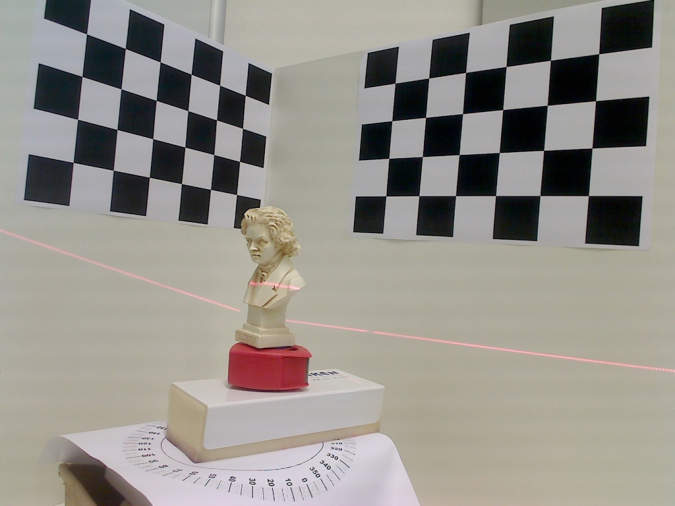
\includegraphics[width=.31\linewidth]{figures/difference-1}
 \label{subfigure:diff-A}} \hfill
\subfigure[$B$]
{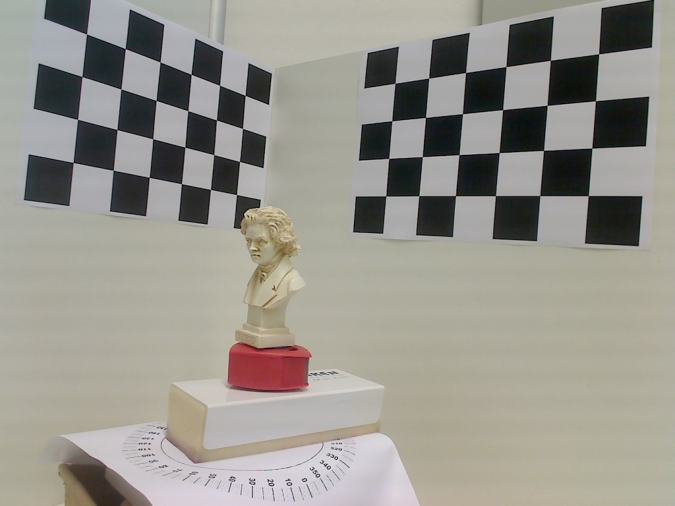
\includegraphics[width=.31\linewidth]{figures/difference-2}
\label{subfigure:diff-B}} \hfill
\subfigure[$C$]
{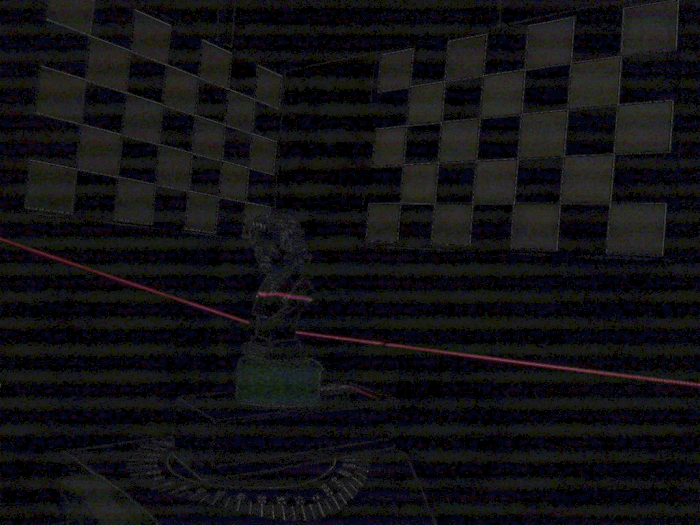
\includegraphics[width=.31\linewidth]{figures/difference-3}
\label{subfigure:difference-C}} \hfill
\label{figure:difference-image}
\caption{Using Image Difference to Find the Laser}
\end{figure}



\begin{figure}[ht!]
\centering
\subfigure[Difference Image]
{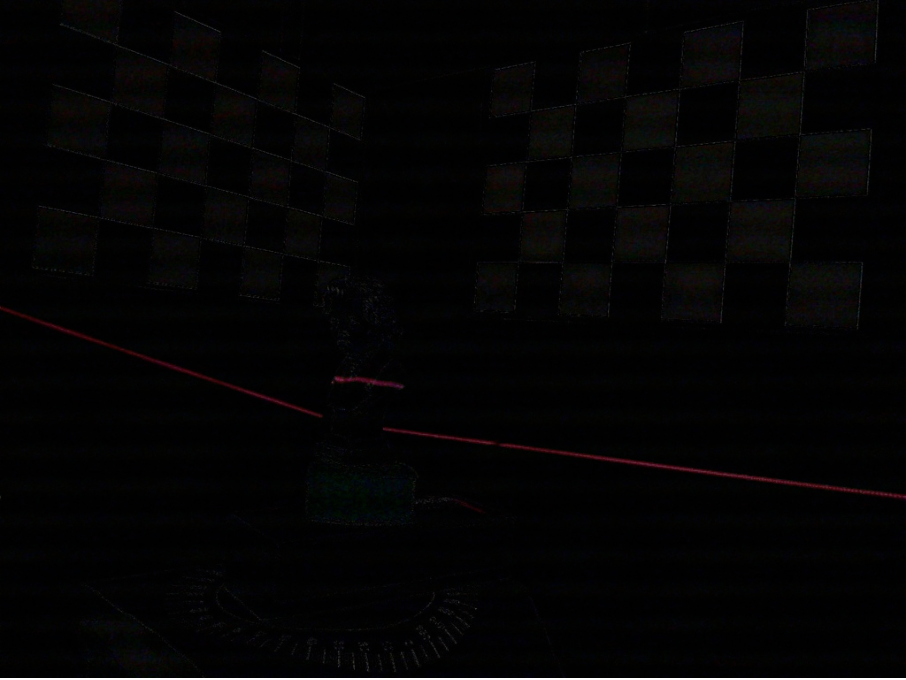
\includegraphics[width=.45\linewidth]{figures/gauss-1}
\label{subfigure:gauss-A}} \quad
\subfigure[Gaussian Smoothened Image]
{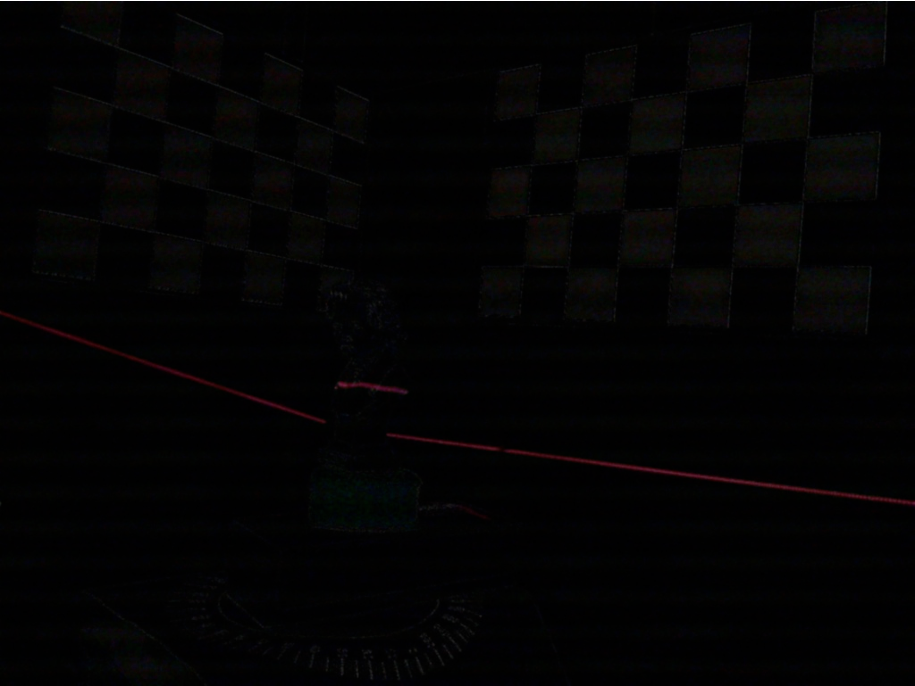
\includegraphics[width=.45\linewidth]{figures/gauss-2}
\label{subfigure:gauss-B}} \hfill
\caption{Gaussian Smoothing the Difference Image}
\end{figure}


\begin{figure}[ht!]
\centering
\subfigure[Image with Outliers]
{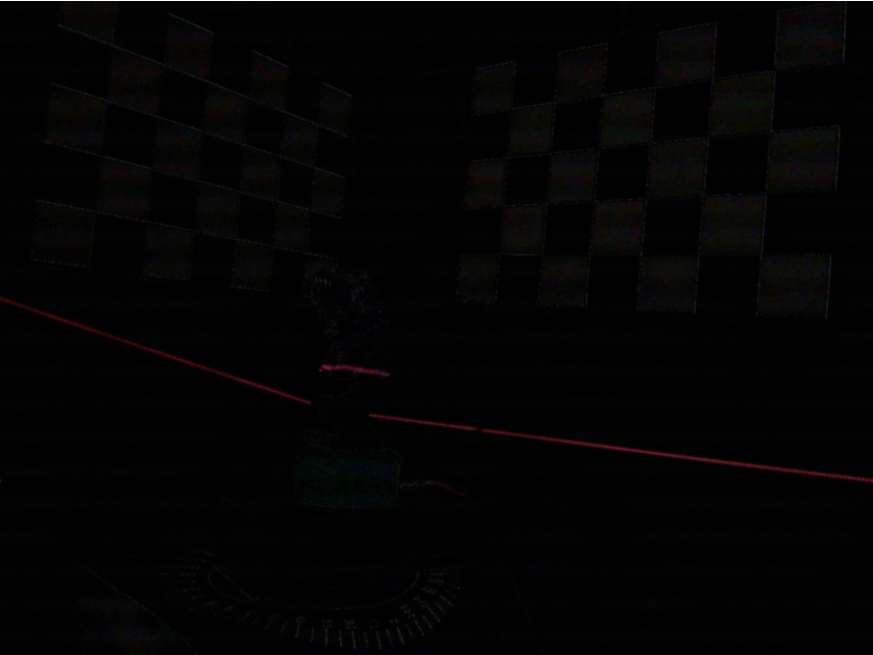
\includegraphics[width=.45\linewidth]{figures/colorthres-1}
\label{subfigure:colorthres-A}} \quad
\subfigure[Image without Outliers]
{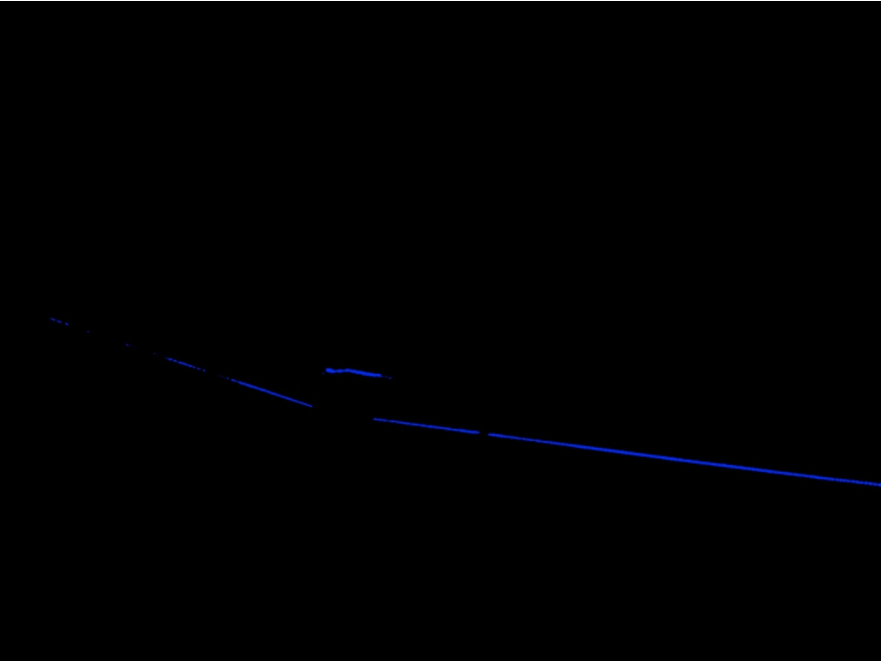
\includegraphics[width=.45\linewidth]{figures/colorthres-2}
\label{subfigure:colorthres-B}} \hfill
\caption{Color Thresholding to Remove Outliers}
\end{figure}

\begin{figure}[ht!]
\centering
\subfigure[Before Transformation]
{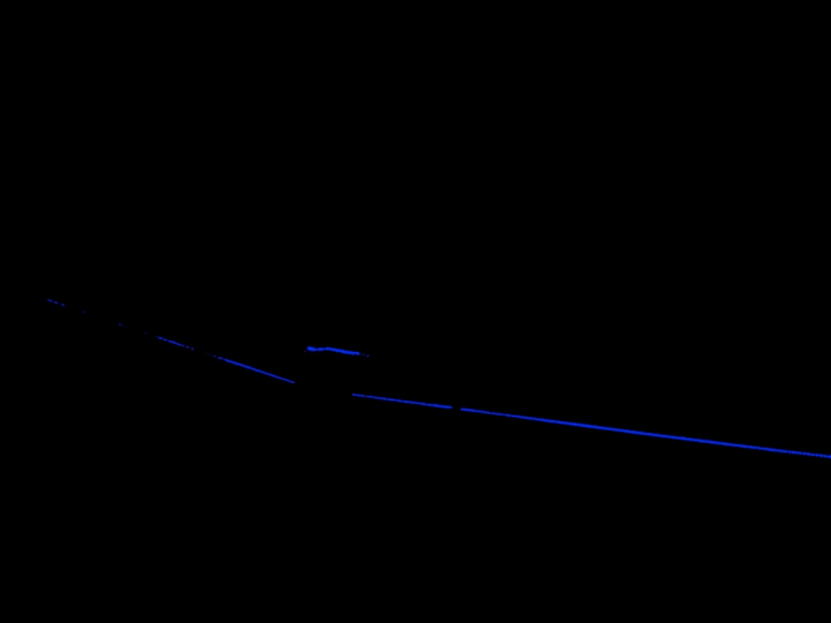
\includegraphics[width=.45\linewidth]{figures/hough-1}
\label{subfigure:hough-A}} \quad
\subfigure[After Transformation]
{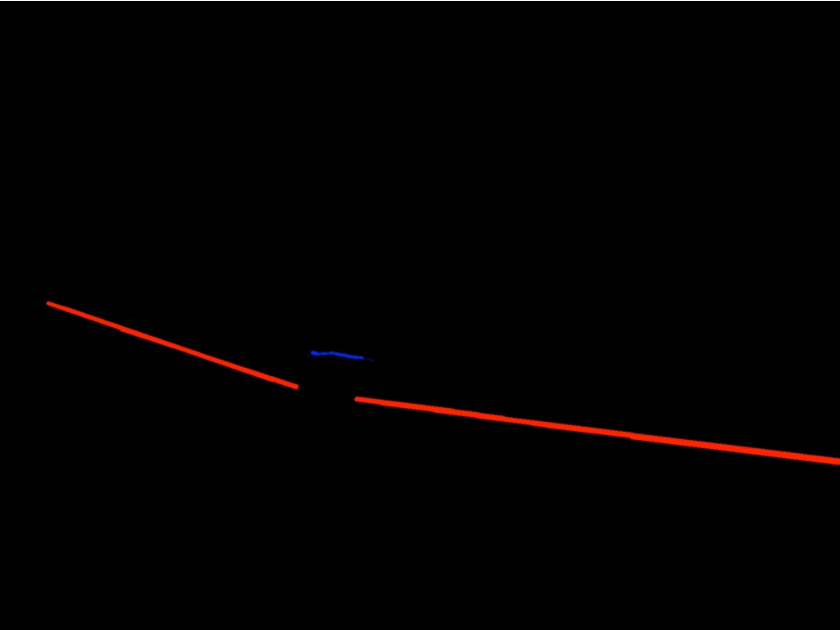
\includegraphics[width=.45\linewidth]{figures/hough-2}
\label{subfigure:hough-B}} \hfill
\caption{Hough Transformation}
\end{figure}




\begin{itemize}
	\item Take a Difference Image to find the Laser
  \item Smoothen the Difference Image
  \item Color Threshold to remove everything else
  \item Apply Hough Transform
  \item Wrap the Points and Return the results
\end{itemize}